\documentclass[11pt]{article}

% include packages
\usepackage{lipsum}
\usepackage[margin=1 in,includefoot]{geometry}
\usepackage[utf8]{inputenc}
\usepackage{hyperref}
\usepackage{multirow}

%%%%%Graphics
\usepackage{graphicx}
\usepackage{float}

%%%%Biblio


%%%%%%%% Header and footer 
\usepackage{fancyhdr}
\pagestyle{fancy}
\fancyhead{}
\fancyfoot{}
\fancyfoot[R]{\thepage}
\renewcommand{\headrulewidth}{0pt}
\renewcommand{\footrulewidth}{1pt}

% deal with hyper link of table of contents and references 
\hypersetup{
    colorlinks=true, %set true if you want colored links
    linktoc=all,     %set to all if you want both sections and subsections linked
    linkcolor=black,  %choose some color if you want links to stand out
}
%%%%%%%%%%%%%%%%%%%%%

% edit start
\begin{document}

% title
\begin{titlepage}
\title{
	{\large People in Ecosystems/Watershed Integration (PEWI)}\\
	{\huge {General Level Index Notes\\}}
	% including logo image
	\begin{figure}[H]
	\centering
	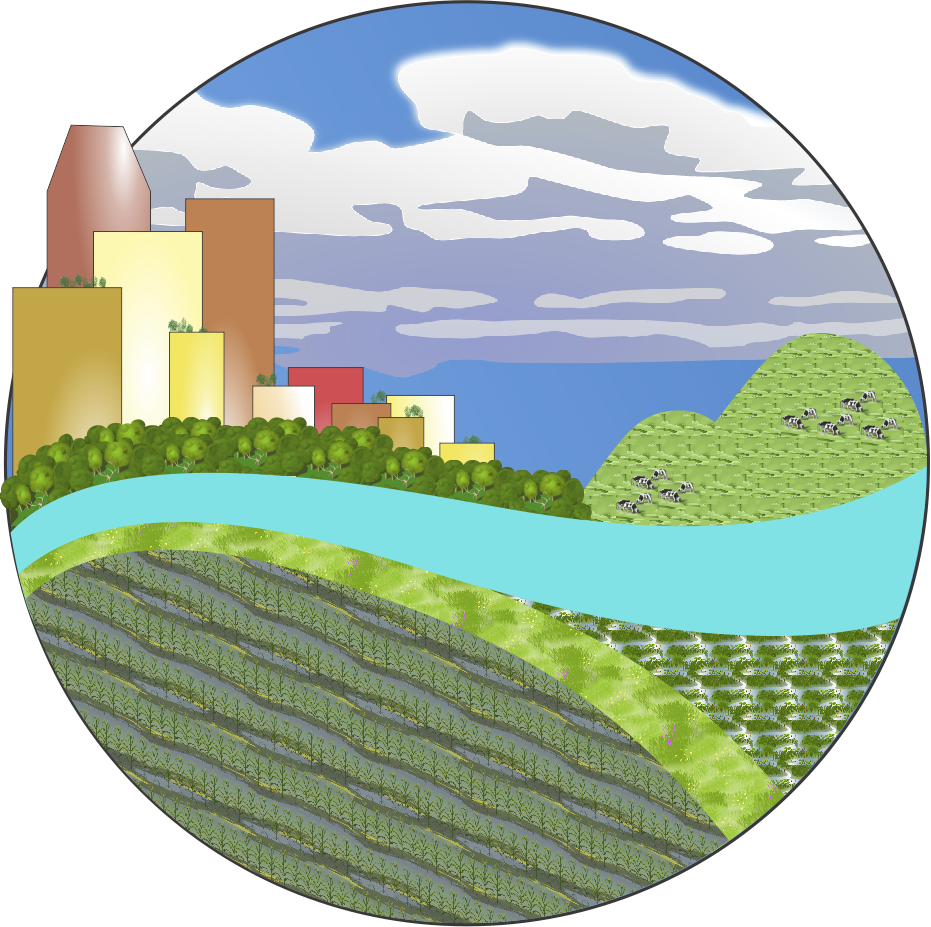
\includegraphics[height=3 in]{../imgs/updatedPewiLogo.png}
	\end{figure}
}
\author{PEWI team}
\date {\today} % date
\maketitle
\thispagestyle{empty} % no page number on cover
\end{titlepage}

% stuff before table of contents
\pagenumbering{roman}
\section*{Summary}
\addcontentsline{toc}{section}{\numberline{}Summary}
This is the document of index. This document includes all descriptions for the general tab.
\cleardoublepage

\section*{Acknowledgements}
\addcontentsline{toc}{section}{\numberline{}Acknowledgements}
Special thanks to many people.
\cleardoublepage


%%%%%Table of content starts here
\tableofcontents
\thispagestyle{empty} % no page number on table of contents page
\cleardoublepage % no other contents on table of contents page

%%% to start page numbers from 1
\pagenumbering{arabic}
\setcounter{page}{1}

% === main contents ===

% Land Use section
\section{Land Use}\label{sec:landuse}
Fifteen land use types are available to choose from in PEWI, including perennial and annual legumes, annual grains, mixed fruit and vegetables, pasture, herbaceous perennials, and woody perennials.

% sub section
\subsection{Conventional Corn}
Corn is an annual grain crop traditionally used for food, animal feed, and biofuel. Corn is currently the most planted field crop in the US, with over 36.4 million hectares (90 million acres) of corn planted every year\cite{1}.  In PEWI, conventional corn land cover assumes conventional tillage and management.

\subsection{Conventional Soy}
Soybeans are an annual nitrogen-fixing legume crop traditionally used for oil, animal feed, food, and industrial products. Soybeans are currently the second-most planted field crop in the US, with 31.4 million hectares (77.5 million acres) of soybeans planted every year\cite{2}.  In PEWI, conventional soybean land cover assumes conventional tillage and management. 

\subsection{Conservation Corn}
Corn is an annual grain crop traditionally used for food, animal feed, and biofuel. Corn is currently the most planted field crop in the US, with over 36.4 million hectares (90 million acres) of corn planted every year\cite{3}.  In PEWI, conservation management assumes use of "no-till," cover crops, grassed waterways and/or buffers, as well as contouring and/or terracing where appropriate to the location (i.e. downhill slopes above 2\% elevation grade).

\subsection{Conservation Soy}
Soybeans are an annual nitrogen-fixing legume crop traditionally used for oil, animal feed, food, and industrial products. Soybeans are currently the second-most planted field crop in the US, with 31.4 million hectares (77.5 million acres) of soybeans planted every year\cite{4}.  As legumes, they fix nitrogen (N2) from the atmosphere, converting it into plant-available ammonia (NH3). Conservation management assumes use of "no-till," cover crops, grassed waterways, and/or buffers, as well as contouring and/or terracing where appropriate to the location.

\subsection{Alfalfa}
Alfalfa is perennial legume traditionally hayed and used as forage for livestock. Approximately 7.3 million hectares (18 million acres) of alfalfa are harvested in the U.S. each year\cite{5}.  On average, three to five cuttings can be taken per year.\cite{6}

\subsection{Mixed Fruit and Vegetables}
The mixed fruit and vegetable land cover in PEWI is based on an equal distribution of four crops: strawberries, grapes, green beans, and squash. Mixed fruit and vegetable land cover in PEWI assumes effective management practices as noted by Taber.\cite{7}

Mixed fruit and vegetable land-use assumes two phosphorus fertilizer methods in equal proportion: surface application with no incorporation and incorporation within one week.\cite{8} 

\subsection{Grass Hay}
Grass hay is a perennial crop traditionally grown and bailed for livestock feed. Over 15 million hectares (38 million acres) of hay, excluding alfalfa hay, are harvested annually in the United States. On average, three cuttings can be taken per year.\cite{9} 

\subsection{Switchgrass}
Switchgrass is a native, herbaceous, low-input perennial crop that can be harvested for biofuel. It is adaptable to many soil types.

\subsection{Permanent Pasture}
Permanent pasture in PEWI is alfalfa or grass hay grazed by cattle for the typical 200 day grazing season from April 15 to November 1.\cite{10}

\subsection{Rotational Grazing}
Rotational grazing is alfalfa or grass hay grazed by cattle for the typical 200 day grazing season from April 15 to November 1, strategically rotated across paddocks for even grazing.\cite{11}

\subsection{Wetland}
Wetlands historically covered 89 million hectares (221 million acres) of what is now the contiguous United States.\cite{12}  Between the years 1780 and 1980, the states of Iowa, Missouri, Illinois, and Indiana underwent an 85 percent decrease of wetland acreage.\cite{13}  The native wetland ecosystem is a rich habitat for a diversity of organisms and provides many benefits through water filtration and retention, soil and nutrient retention, and carbon sequestration. Wetlands also hold potential as a venue for tourism, recreation, and hunting.\cite{14} In PEWI, the benefits of restored wetlands are maximized by using Strategic Wetland areas.

\subsection{Prairie}
The Prairie land cover in PEWI consists of a diverse mix of tall grass prairie native to Iowa.\cite{15}  Less than 1 percent of the historical 97 million hectare (240 million acre) extent of tall grass prairie remains.\cite{16}  In Iowa, less than 0.1 percent of the original 12.1 million hectares (30 million acres) remain.\cite{17}
The native prairie ecosystem is a rich habitat for a diversity of organisms and provides many benefits through water filtration and retention, soil and nutrient retention, and carbon sequestration. Prairies also hold potential as a venue for tourism, recreation, and hunting.\cite{18}  Restored prairie may also be a source for valuable prairie seeds and native grasses for biomass.
\subsection{Conventional Forest}
PEWI conventional and conservation forest land covers assume appropriate tree species selection for each soil type. Information on specific tree species is available through the Iowa Woodland Suitability Composite.\cite{19}

In practice, conventional forests are managed on an ad hoc basis. The forest is periodically clearcut or high-graded, in which the most valuable trees are removed. Strategy is not customized based on the historical composition or structure of forests in the area.\cite{20}. 


\subsection{Conservation Forest}
	PEWI conventional and conservation forest land covers assume appropriate tree species selection for each soil type. Information on specific tree species is available through the Iowa Woodland Suitability Composite.\cite{21}

Conservation forest in PEWI assumes management with regard to historically relevant compositional and structural diversity using a variety of strategic techniques. These may include uneven-aged management including gap or patch cuts, even-aged management including shelterwood or crop tree release, and other techniques such as timber stand improvement, prescribed burning and/or tactical grazing, and removal of invasives.\cite{22}  It also assumes "management of coarse woody debris, mast-bearing trees, and sensitive areas such as riparian zones, ephemeral ponds, and rock outcrops." .\cite{23}


\subsection{Short-Rotation Woody Bioenergy}
Short rotation woody crops are fast-growing trees, such as eucalyptus, poplar, and willow, grown for bioenergy and biofuel. In PEWI, aspen is used on a 10-year rotation.

% Physical Features section
\newpage
\section{Physical Features}\label{sec:physicalfeatures}
In the Physical Features tab, you'll find information on topography, soil properties, subwatershed boundaries, and strategic wetland areas. These properties can help you strategize the placement of land uses. Physical features influence the Ecosystem Services gained from each land cover choice, from soil and water quality improvement to yield.

% sub section
\subsection{Topographic Relief}
This feature shows the elevation grade, or slope, of each cell of PEWI. Land use covers perform differently under different elevations, and the topographic map can help explain results and inform location-specific land use choices. The lightest color represents the shallowest slope, and the darkest color represents the steepest slope.

\subsection{Flood Frequency}
\raggedright
This feature shows the frequency of flooding for each PEWI grid cell, as found in the Iowa Soil Properties and Interpretations Database (ISPAID) Soil Survey.\cite{25}  Flooding categories are defined below, according to the ISPAID manual. In PEWI, flooding frequency is incorporated into yield calculations: yield is determined as per ISPAID calculations as a function of CSR2 results. The CSR2 formula is CSR2 = S-M-W-F-D+/- EJ, where F is the field condition including ponding and flooding properties, among other factors.\cite{26}  See the Yield tab for more information.
\begin{itemize}
\item NONE	=	0	=	Flooding is not probable.
\item RARE	=	10	=	Flooding is unlikely but possible under unusual weather conditions.
\item OCCAS	=	20	=	Flooding occurs on an average of 50 times or less in 100 years.
\item FREQ	=	40	=	Flooding occurs on an average of more than 50 times in 100 years.
\item PONDED	=	50	=	Standing water on soils in closed depressions.  Unless the soils are artificially drained, the water can be removed only by percolation or evapotranspiration.  (Ponded is for short duration unless otherwise specified).
\end{itemize}

\subsection{Strategic Wetlands}

There are 20 strategic wetlands in PEWI. These include “prairie potholes” in the lower lobe of the watershed that are prone to flooding, but have poor drainage, and shallow areas along the river or a tributary that would regularly have high moisture content in the soil. Utilizing strategic wetlands by planting Wetland in these areas leads to a significant improvement in ecological services.

Wetlands including prairie pothole wetlands and stream buffer wetlands provide native habitat for amphibians, invertebrates, and birds including ring-necked pheasants and mallards,\cite{27}  increasing biodiversity and game wildlife services. It also curbs nitrate pollution; for subwatersheds with at least one strategic wetland, nitrate loss is cut by 52 percent.\cite{28}

\subsection{Subwatershed Boundaries}
This feature depicts the boundaries of each subwatershed, which are important in water runoff patterns influencing nitrate loss. Subwatershed boundaries were realistically calculated based on topographic modeling for the watershed. 

\subsection{Drainage Class}
This feature shows the relative drainage of each pixel in PEWI. Drainage classes are defined below, according to the Iowa Soil Properties and Interpretations Database (ISPAID) manual.\cite{29}  In PEWI, drainage class influences phosphorus, and ISPAID yield values incorporate drainage class information; for more information see the Yield tab.\cite{30}  The subsurface drainage component (SDC) of the phosphorus delivery calculation is a function of flow factor (FF), which is dependent on drainage class. Additionally, the runoff component of the phosphorus calculation incorporates runoff curve numbers based on hydrologic group. See the Phosphorus Tab and Hydrologic Group Tab for more information. 
\begin{itemize}
\item E	=	10	=	Excessive
\item E-SE	=	15	=	Excessive-Somewhat excessive
\item SE	=	20	=	Somewhat excessive
\item SE-W	=	25	=	Somewhat excessive-Well
\item W	=	30	=	Well
\item W-MW	=	35	=	Well-Moderately well
\item MW	=	40	=	Moderately well
\item MW-SP	=	45	=	Moderately well-Somewhat poor 
\item SP	=	50	=	Somewhat poor
\item SP-P	=	55	=	Somewhat poor-Poor
\item P	=	60	=	Poor
\item P-VP	=	65	=	Poor-Very poor
\item VP	=	70	=	Very poor
\end{itemize}

\subsubsection{Hydrologic Group}
Hydrologic groups are used to estimate runoff from precipitation. They influence runoff curve numbers (RCN) for each land use type, which are used to calculate the runoff component of phosphorus transport. Soils are classified into one of four hydrologic groups based on drainage class and other attributes such as texture.\cite{31} 

\subsection{Yield Overlay Maps}
Soybean, Mixed Fruit and Vegetables, Cattle, Alfalfa, Grass Hay, Switchgrass, Wood, and Short-Rotation Woody Biomass. Each yield type has a yield base rate based on soil type. The colors for each map on the map keys are the same colors as the ones on the maps to help the User to strategically place landuse types on the map. In addition to the yield base rates being on the Map Keys, Precipitation Tables are provided to show yield precip factors at different precipitation levels. 

\subsection{Soil Class}
There are thirteen soil classes in PEWI. Each soil class has its own set of properties, including percent slope, flood frequency, drainage class, hydrologic group, soil texture, Corn Suitability Rating, and taxonomic classification. The class of a soil can tell you about its physical and chemical composition, which influences its behavior and production capacity in various situations. 

\subsection{Soil Texture}
Texture refers to the composition of the soil, including organic matter content and particle size distribution. Abbreviations for texture types used in the ISPAID are below.
\begin{itemize}
\item C                =    Clay
\item CL              =    Clay loam
\item CN-SIL       =    Channery silt loam
\item CO-SICL     =    Cobbly silty clay loam
\item CS              =    Coarse sand
\item CSL            =    Coarse sandy loam
\item FS              =    Fine sand
\item FSL            =    Fine sandy loam
\item GR-SL        =    Gravelly sandy loam
\item L                =    Loam
\item LS              =    Loamy sand
\item LFS            =    Loamy fine sand
\item MK             =    Muck
\item MK-SICL    =    Mucky silty clay loam
\item MK-SIL       =    Mucky silt loam
\item S                =    Sand
\item SIC             =    Silty clay
\item SICL           =    Silty clay loam
\item SIL             =    Silt loam
\item SL              =    Sandy loam
\item SP              =    Sapric
\item VFSL          =    Very fine sandy loam
\end{itemize}
A table of soil texture by soil type is below.

\begin{center}
\begin{tabular}{ |c|c|c|c| } 
\hline
County & ISPAID Soil Type & Texture \\
\hline
\multirow{3}{7em}{Boone County} & Clarion 138B & L \\ 
& Buckney 1636 & FSL \\ 
& Canisteo 507 & SICL \\ 
& Coland 135   & CL  \\
& Nicollet 55  & L   \\
& Okoboji 90   & MK-SIL \\
\hline
Jasper County & Downs 162D2 & SIL \\
& Gara-Armstrong 993E2 & L \\
& Ackmore-Colo 5B & SIL\\
& Tama 120C2 & SICL \\
& Tama 120B  & SICL \\
& Muscatine 119 & SICL \\
& Nodaway 220 & SIL \\
\hline
\end{tabular}
\end{center}

\subsection{Corn Suitability Rating}
The CSR2 calculates the corn suitability value as:
CSR2 = S-M-W-F-D +/- EJ
\begin{itemize}
\item Where S is the taxonomic subgroup class of the soil 
\item M is the family particle size class (soil particle composition)
\item W is a function of the soil’s water holding capacity
\item F is the field condition factor, including slope, erosion class, flooding, and topsoil thickness
\item D incorporates soil depth and “T factor,” or soil loss tolerance
\item EJ is an expert judgment factor accounting for series abnormalities such as textural extremes or high bulk density.\cite{32} 
\end{itemize}

% Precipitation section
\newpage
\section{Precipitation}
Precipitation is based on historical annual precipitation data from Iowa to simulate climate variability. Scenarios are broken into three categories. 
\begin{itemize}
  \item The Dry category includes the 62.4 cm/yr (24.58 in/yr) scenario, with a probability of 5\%, and the 71.6 cm/yr (28.18 in/yr) scenario, with a probability of 15\%. 
  \item The Normal category includes the 77.2 cm/yr (30.39 in/yr) scenario, with a probability of 15\%, the 81.7 cm/yr (32.16 in/yr) scenario, with a probability of 15\%, and the 87.2 cm/yr (34.34 in/yr) scenario, with a probability of 15\%.
  \item The Wet category includes the 92.6 cm/yr (36.47 in/yr) scenario, with a probability of 15\%, and the 114.6 cm/yr (45.1 in/yr) scenario, with a probability of 5\%.
\end{itemize}

In PEWI, the level of precipitation influences water quality and soil quality metrics including nitrate and phosphorus runoff, gross erosion, and sediment transport. This is because improved water flow carries a greater quantity of soil and nutrients downstream. Extremes in precipitation also decrease yield for annual crops, mixed fruits and vegetables, alfalfa, grass hay, switchgrass, permanent pasture, and rotational grazing.\cite{33}  Calculations for yield for each land use can be found in the corresponding yield tab.


% Management Practices section
\newpage
\section{Management Practices}
Here you’ll find information on management practices used in PEWI’s calculations.

\subsection{Crop Rotation}
Erosion, phosphorus, and sediment are influenced by Cover Management Factor, which depends on both the preceding land cover and the current land cover. To reduce this factor, try using a rotation with a conservation or perennial crop.

% Modules section
\newpage
\section{Modules}
The scientific modules in PEWI display ecosystem service scores, the benefits that the watershed provides to people. PEWI tracks ecosystem services in four categories: 
\begin{itemize}
\item Habitat
\item Soil Quality
\item Water Quality
\item Yield
\end{itemize}
\subsection{Habitat}
This category includes two Habitat metrics. Providing habitat to a multitude of species is important for water quality, nutrient recycling, pollination, and biocontrol, including suppression of pests that decrease crop production. A highly diverse ecosystem is also more highly adaptable to regional and global stressors and extreme disturbances, such as fires or flooding.

\subsubsection{Biodiversity}
The biodiversity indicator presents a relative measure of how well a landscape pattern maintains habitat suitability at the watershed scale for native species, based on landscape configuration and composition.  According to Fischer, Lindenmayer, and Manning, native vegetation and similar vegetation structures support high biodiversity.\cite{34}  Biodiversity is important for maintenance of water quality and for biocontrol, including suppression of pests that decrease crop production.\cite{35} 

\subsubsection{Game Wildlife}
  The Game Wildlife index is adjusted to reflect greater need to reach a minimum threshold area for appropriate land-use types for the habitat of each game species, including mallard duck, wild turkey, ring-neck pheasant, bobwhite quail, and sport fish. 
  
\subsection{Soil Quality}
 Soil quality is important for agricultural production and ecosystem health. PEWI monitors two metrics of soil quality: carbon sequestration and erosion prevention. Soils have an immense carbon-holding capacity and, through the actions of plants and microbes, can reduce air pollutant levels. Protecting soils can also minimize erosion, which can diminish crop productivity and deteriorate aquatic stream habitat.\cite{36} 
 
\subsubsection{Carbon Sequestration}
Carbon sequestration involves removing carbon dioxide from the air and storing it long-term in the soil. This is beneficial for long-term soil health, plant nutrient availability and sustained productivity, and control of atmospheric carbon dioxide. 
 
\cleardoublepage
\newpage

\subsubsection{Erosion Control}
The Erosion Control module is based on guidelines from the 2004 Iowa Phosphorus Index. Gross Erosion is the soil loss per year from ephemeral gully erosion, rill erosion, and interrill erosion; a high gross erosion corresponds to a low soil retention, and low gross erosion to a high soil retention. Excessive soil erosion has been shown to decrease soil and water quality, leading to diminished crop productivity and deterioration of aquatic stream habitat.\cite{36}

\subsection{Water Quality}
Water quality is a salient issue for Corn Belt states and other agricultural regions. PEWI tracks three metrics of water quality: nitrate, sediment, and phosphorus. Nitrate-N concentrations in drinking water exceeding the Environmental Protection Agency’s National Regulation limit of 10 mg/L can lead to negative health effects, including blue baby syndrome.\cite{37}  Downstream, nitrate-N loading also creates hypoxic (low-oxygen) zones in gulf regions, leading to loss of marine life.\cite{38}  Sediment delivery impacts water quality both locally and downstream.\cite{39} Phosphorus loss impacts local producers who incur expenses of phosphorus fertilizer application, regional aquatic ecosystems and human economy through freshwater eutrophication, and distant scales through gulf hypoxia.\cite{40} 

\subsubsection{Nitrate Retention}
Nitrate pollution is a well-known public health problem that negatively affects human health when exceeding a contamination level of 10 mg L-1 in drinking water, which is the limit established in the National Primary Drinking Water Regulations.  It also harms aquatic ecosystems by depleting oxygen in the Gulf of Mexico.\cite{41}

\subsubsection{Phosphorus Retention}
Phosphorus transport from fields to surface water can threaten aquatic species and human economy due to aquatic eutrophication. In PEWI, Phosphorus Retention is the indexed inverse of annual in-stream phosphorus loading, with high phosphorus runoff corresponding to low phosphorus retention, and vice versa.

\subsubsection{Sediment Control}
Sediment transport can adversely affect water quality both at the local level and downstream. Sediment control is the indexed inverse of annual in-stream sediment delivery. 

\subsection{Yield}
Yields are based on modifications to Corn Suitability Rating, determined by the CSR2 from Iowa State University. The CSR2 assigns a corn suitability rating to each soil type in Iowa, and this data is incorporated into PEWI grid cells. Yields from other crops are estimated as a proportion of corn yield values. 

\subsubsection{Corn Yield}
The Corn Grain yield in PEWI assumes high-level management, and no difference between yield in conventional and conservation systems. Corn grain yield is based on the Iowa Soil Properties and Interpretations Database (ISPAID) equation of Corn Yield = (1.6 * Corn Suitability Rating) + 80, and multiplied by a conversion factor of 0.0254 Mg/bu.\cite{42}  
 Total production is given by the product of the yield on a per-unit basis and the area of the grid cell, summed over the entire watershed. 
 
\subsubsection{Soybean Yield}
Soybean yield is based on the Iowa Soil Properties and Interpretations Database (ISPAID) equation of Soybean Yield = 0.29 * Corn Yield. Total production is given by the product of the yield on a per-unit basis and the area of the grid cell, summed over the entire watershed. 

\subsubsection{Alfalfa Hay Yield}
Alfalfa Hay yield is based on the Iowa Soil Properties and Interpretations Database  (ISPAID) equation of YBij[Alfalfa] = DFij * Corn Yield multiplied by a conversion factor from tons to megagrams and with a minimum of 8.07 Mg/ha yr.\cite{43} 

DFij is a drainage factor equal to:
\begin{itemize}

\item 0.028 for soils with Drainage Class values of 10-35, as well as most soils with Drainage Class values of 40
\item 0.026 for soils with Drainage Class values of 45-50, as well as two soils with Drainage Class values of 40
\item 0.021 for soils with Drainage Class values of 55-70

\end{itemize}

Total production is given by the product of the yield on a per-unit basis and the area of the grid cell, summed over the entire watershed. 

\subsubsection{Grass Hay}
Grass Hay yield is based on the Iowa Soil Properties and Interpretations Database (ISPAID) equation of YBij[GrassHay] = DFij * CornYield multiplied by a conversion factor from tons to megagrams and with a minimum of 8.07 Mg/ha yr.\cite{43} 

DFij is a drainage factor equal to:

\begin{itemize}

\item 0.028 for soils with Drainage Class values of 10-35, as well as most soils with Drainage Class values of 40
\item 0.026 for soils with Drainage Class values of 45-50, as well as two soils with Drainage Class values of 40
\item 0.021 for soils with Drainage Class values of 55-70

\end{itemize}

Total production is given by the product of the yield on a per-unit basis and the area of the grid cell, summed over the entire watershed. 

\subsubsection{Cattle Yield}
Cattle yield is based on the Iowa Soil Properties and Interpretations Database (ISPAID) equation of Alfalfa-Grass Hay Yield, with a conversion from Alfalfa-Grass yield to head of cattle.

\subsubsection{Mixed Fruit and Vegetable Yield}
Yield for mixed fruit and vegetables is determined from an estimate for grapes, strawberries, green beans, and squash, with each grid cell divided evenly among the four crops. 

\subsubsection{Wood Yield}
Wood production is based on estimates generated using the 2007 Iowa Woodland Suitability Composite.\cite{44} Yield estimates assume appropriate selection of tree species for a given location. A 30\% reduction in wood production estimates for conservation forest is applied to account for differences in management.

\subsubsection{Switch Grass Yield}
Switchgrass biomass yields are based on a modification to Iowa Soil Properties and Interpretations Database (ISPAID) corn suitability ratings.\cite{45}

\subsubsection{Woody Biomass}
Woody biomass yield estimates are based on a 10-year aspen biomass of 224 Mg/ha.\cite{46}  Annual production assumes temporally spaced plantings such that a constant 22.4 Mg/ha is harvested each year.

\newpage

\section{Functionality}
This section describes how to navigate the PEWI application, including play mode options and watershed editing tools.

\subsection{Navigating the PEWI Workspace}
Opening Sandbox or playing a PEWI Level brings you to the PEWI Workspace. In the workspace, there are many tools that you can use to edit the watershed and monitor ecosystem services.

\subsubsection{Tool Panel}
The tool panel has seven features to use in designing your watershed. The Land Use tab includes 15 land cover options to use in your watershed, ranging from annual and perennial crops to pasture, forests, and native land cover.

The Precipitation tab shows the precipitation for each year. PEWI simulates real life by choosing randomly from seven precipitation levels. To override the presets, select a precipitation level from the drop-down menu.

The Years tab allows you to add another year of simulation to your watershed. Some of the impacts of land use choices vary with weather or previous practices. You can explore these effects by playing across multiple years.

The Indicator Tab includes overlay maps for Nitrate, Erosion, and Phosphorus risk. You can edit the land use while in overlay mode to target a specific risk area.

The Physical Features tab includes five watershed behavior overlay maps displaying flood frequency, strategic wetland areas, subwatershed boundaries, drainage class, and soil class. You can edit the land use while in overlay mode to target a specific region.

The Yield Tab allows you to strategically place landuse types on the map, by providing information for each yield type and their respective yield base rates based off soil type. To learn more about this feature, check out the Yield Tab video.

The buttons located above the Toolbar are for placing landuse types on the map. The leftmost button is the individual brush, allowing you to paint one landuse type at a time. The middle button allows you to paint multiple tiles at once by dragging and clicking the corners. The arrow button is the Undo button, allowing you to undo previous changes. Any amount of previous changes can be undone. You can also undo changes by pressing the "U" hotkey on the keyboard. 

\subsubsection{Results Panel}
The results page provides data visualization and numerical results for your watershed design.

\paragraph{Land Use Graph}
The first circle graph gives the percent of the watershed you’ve devoted to each of the land uses. Scroll over the graph or the legend on the right to view the quantitative data for that land use. Use the up and down arrows to switch between List view and Category view. List view displays each land use individually. Category view groups land uses into seven categories: annual grain, annual legume, mixed fruit and vegetables, pasture, non-pasture perennial herbs, perennial legume, and perennial wetland. Use the arrows to switch between years. 

\paragraph{Ecosystem Services Graph}
The ecosystem services radar plot shows the zero-to-100 score of ecosystem services pertaining to water quality, soil health, and habitat. A watershed design with high scores in many ecosystem services will produce a radar plot shape with a large area, while a watershed design with low ecosystem service scores will produce a smaller shape. 

\paragraph{Precipitation Graph}
The precipitation graph shows the amount of precipitation for each year of the simulation. 

\paragraph{Data Sheet}
Click on the abacus icon at the top of the Results page to access the data tab with two numerical tables. Both tables provide three metrics: the zero-to-100 scale used in the Scores tab, English units, and metric units. The first table gives the percent area of each land use by year, and the second gives ecosystem service scores by year. At the bottom of the page are precipitation data and strategic wetland use for each year. 

\subsubsection{Comment Panel}
Click the comment bubble to show or hide the comment panel. In Level mode, the comment panel will show instructions for completing the next objective in the level. 

\subsubsection{Index Information Box}
The Index Information Box is located at the bottom right portion of the screen. Each tab is given particular information about their intended usage and each individual feature for each tab is given some information in the Index Box and where to learn more, by directing the User to its respective Index entry. Every tab, from the Landuse Tab to the Yield Tab has information. Check them out! 

\subsubsection{View Perspective}
Press or hold D to rotate the watershed clockwise.
Press or hold A to rotate the watershed counterclockwise.
Press or hold W to pivot your viewpoint toward the horizon (flat)
Press or hold S to pivot your viewpoint toward the perpendicular
Right click to rotate the canvas with your mouse.

Use the up and down arrow keys to zoom in and out.
Use the left and right arrow keys to pan left and right.

Press T to toggle 3-D topographical view.

Press E to reset the camera position to default.

\subsubsection{Save Watershed}
Click the download icon in the upper right-hand corner to save your watershed to your computer. Upload to continue with your design.

\subsection{Main Menu}
Select Sandbox to explore the watershed on your own.
Select Play to play an interactive PEWI level.
Select Utilities to design a level, set up Multiplayer Mode, or aggregate Multiplayer Maps.
For more information, see the Levels tab and Multiplayer Mode tab.

\subsection{Guided Play}
PEWI comes with predesigned, thematic levels, ranging from introductory to complex. The N-Factor (Nitrogen) set focuses on the interaction between nitrate levels, physical features, land uses, and other ecosystem service scores. The P-Factor (Phosphorus) focuses on improving phosphorus, sediment, and erosion levels. The B-Factor (Biodiversity) focuses on habitat variety and suitability.

To create your own level, choose Design a Level from the Utilities menu. You can write a customized lesson with your own objectives and board presets.

\subsection{Multiplayer Mode}
PEWI offers a Multiplayer Mode. Under Utilities, click on the "Set-Up Multiplayer" button. In Multiplayer Mode, up to 6 Players can be added. Click on the Player numbers to draw out boundaries for each Player on the map with the brush tools.

You can also merge and combine Player boundaries and add and remove Players. Once finished, press "V" to download a Multi-Map file. Return to sandbox and click on the down arrow on the upper right part of the screen. Click on Upload and select a Player from your map files. In this case, Player 1 will be given only their boundaries drawn out for them to paint landuse types on. Scores in the Results are adjusted for these sections.

You can continue to adjust any Player maps as seen fit. Once finished, hit download to update the maps. To see all of the maps put together at once, go to "Utilities" and "Aggregate Multi-Maps". Add the files that have been changed and download the aggregate maps. Go back to "Sandbox" and upload the combined map file.

\subsection{Pause Menu}
The Pause Menu can be accessed by pressing the "Escape Key" Clicking on the Index will take you to the various Index Entries, where you can learn about different features of PEWI with videos The "Instructor Options" feature can also be accessed where customizations can be made and are further explored in the "Instructor Options" video The final part of the Pause Menu is the "Main Menu" feature, where you can go back to PEWI's main menu.

\subsection{Hover Information}
Specific information can be shown when hovered over tiles on the map. Each map when hovered over will display the tile's coordinates, the Land Cover that is currently being placed on the map, Precipitation level, and Soil Type. On some maps, there are some additional bits of information when hovered over. For the Nitrate, Erosion, and Phosphorus Maps, raw scores will show up that correspond to their map keys. Strategic Wetlands and Subwatershed Boundaries have their sections appear, while Flood Frequency, Drainage and Soil Class have their map key information appear. Yield maps all have their raw scores appear as well. Hover information displayed can be customized in the Instructor Options page and can be toggled on and off accordingly.  

\subsection{Hotkeys}
\begin{itemize}
\item Shift + Click	Fill the watershed with the selected land type
\item E	Reset camera position
\item Escape	Access Pause Menu
\item R	Randomize all land use types
\item T	Toggle topographical view
\item U	Undo previous land change
\item O	Toggle previous overlay
\item B	Toggle recording feature
\item V	Create multiplayer maps in multiplayer utility
\item D	Rotate clockwise
\item A	Rotate counterclockwise
\item W	Pivot toward the horizon (flat)
\item S	Pivot toward the perpendicular
\item Q	Toggle Flying Mode
\item Use the up and down arrow keys to zoom in and out
\item Use the left and right arrow keys to pan left and right
\item Right Click	Rotate watershed with your mouse
\end{itemize}

\subsection{Hotkey Customization}
By pressing the Esc Key and going to Instructor Options, a list of Hotkeys is available with their default settings. However, the hotkeys can be customized and adjusted as much as possible, with the option of having two hotkeys per feature. You can also reset the hotkeys to bring them back to their default settings. 

\subsection{Randomization}
Press "R" to randomize the landuse tiles on the watershed. The watershed can be randomized an infinite number of times. Press the Esc key to go to Instructor Options, where you can turn off landuse types. By turning off Conventional Corn, the landuse type will no longer appear when randomized. This applies for any other landuse types that are turned off. Landuse types can be turned back on and put back into randomization through the Instructor Options as well. 

\subsection{Undo Function}
In PEWI, there is an undo function that allows you to undo changes to the map, such as painting tiles or randomizing the map. Once you want to make changes to your previous edits to the map, click on the undo button, located next to the paint brush buttons above the tool box. You can also undo your changes by pressing the "Undo Hotkey" which is "U" on the keyboard. You can undo up to your oldest change to the map. The undo hotkey also extends to painting multiple tiles at once. 

\subsection{Print Function}
You can print your maps, results, and much more with Pewi. Activate the Print function by pressing "P" on the keyboard and select what you want to be printed out on a PDF. There are plenty of categories to choose from to print, including: Landuse Type Maps for set years, results, levels maps, and much more. Buttons such as "Select All" and "Reset" can help you choose. Once finished, you can click "Preview PDF" to see what will be on your PDF and then "Download" when ready. You can then print out your PDF once you save it. When you're finished, click "Exit". 

\subsection{Record}
By pressing B, you can record your actions with PEWI. The record feature will keep track of all actions. When you're done recording, press B again to save what was recorded. If you want to see your recording, go back to the main menu and click on "Utilities", then "Run User Simulation" where you can upload your recording. Once clicking "Click here to begin Simulation", you can view your recording. A bar at the bottom left of the screen will show the recording's progress and it's possible to fast forward and rewind. Once finished, you can replay or return to the Main Menu. 

\subsection{About}
People in Ecosystems/Watershed Integration (PEWI) is a simple web-based educational game designed to provide a scientific platform for teaching, discussing, and evaluating the tradeoffs associated with agricultural land use and management. Players iteratively manipulate land use annually for three years in a virtual 6000 acre watershed to meet a variety of goals. The tool computes a variety of results, including agricultural yields, soil erosion, stream pollution, and wildlife habitat.

PEWI v3 is developed and maintained to be compatible with Google Chrome (versions 49+), Internet Explorer (versions 11+), Mozilla Firefox (versions 47+), and Safari (versions 9.1+).

PEWI is a product of Iowa State University Department of Natural Resource Ecology and Management. The product license can be found here. Members of the PEWI development team were Lisa Schulte Moore, Assata Caldwell, Carrie Chennault, Justin Choe, Ryan Frahm, Noah Hagen, Jake Hill, Charles Labuzzetta, Laura Roy, Nancy Shryock, John Tyndall, Robert Valek, and John VanDyk.

PEWI v3 was funded through grants from the Iowa State University Department of Agronomy, McKnight Foundation, and USDA Forest Service.

More information on PEWI, including information on tool development, learning exercises, additional acknowledgements, and how you can contribute can be found at the project website: www.nrem.iastate.edu/pewi. Questions can be sent to pewi@iastate.edu. 

\newpage

% References
\begin{thebibliography}{1}

  \bibitem{1} Thomas Capehart {\em "Corn - Background," USDA Economic Research Service, }July 14, 2016,\url{http://www.ers.usda.gov/topics/crops/corn/background.aspx}

  \bibitem{2}  Mark Ash, Shelbi Knisley {\em "Soybeans and Oil Crops - Background," USDA Economic Research Service}, accessed September 14, 2016, \url{http://www.ers.usda.gov/topics/crops/soybeans-oil-crops/background.aspx}.

  \bibitem{3} Thomas Capehart July 14, 2016, \url{http://www.ers.usda.gov/topics/crops/corn/background.aspx}.

  \bibitem{4}Mark Ash, Shelbi Knisley  "Soybeans and Oil Crops - Background," USDA Economic Research Service,accessed September 14, 2016, \url{http://www.ers.usda.gov/topics/crops/soybeans-oil-crops/background.aspx}.
  
  \bibitem{5}"Crop Production 2015 Summary" (United States Department of Agriculture | National Agricultural Statistics Service, January 12, 2016), \url{http://www.usda.gov/nass/PUBS/TODAYRPT/cropan16.pdf}.
  
  \bibitem{6}Stephen Barnhart, "When to Make First Spring Cut of Alfalfa and Mixed Alfalfa/Grass | Integrated Crop Management," Iowa State University Extension and Outreach, May 13, 2010, \url{http://crops.extension.iastate.edu/cropnews/2010/05/when-make-first-spring-cut-alfalfa-and-mixed-alfalfagrass}.
  
  \bibitem{7}H. G. Taber, "Commercial Vegetable Production – A Small Farm Opportunity?" (Iowa State University Extension and Outreach, 2009), \url{http://ia.foodmarketmaker.com/uploads/0a88216bd7a96e10152b7c7a6891a667.pdf}.
  
  \bibitem{8}Matthew Helmers and Thomas Isenhart, (Iowa State University, personal communication, 2014); Carrie Chennault, "People in Ecosystems / Watershed Integration: Visualizing Ecosystem Services Tradeoffs in Agricultural Landscapes" (Master’s thesis, Iowa State University, 2014), 51
  
  \bibitem{9}Jeff DeYoung, “First-Cutting Hay Sets Tone for Rest of Season,” Iowa Farmer Today, June 1, 2005, \url{http://www.iowafarmertoday.com/news/regional/first-cutting-hay-sets-tone-for-rest-of-season/article_bb73c2ca-df0d-58e0-b7a5-5867b46a93a2.html}.
  
\bibitem{10}Carrie Chennault, "People in Ecosystems / Watershed Integration: Visualizing Ecosystem Services Tradeoffs in Agricultural Landscapes" (Master’s thesis, Iowa State University, 2014), 78; "Custom Grazing Survey 2007: Demographics \& Management Practices," Cattle Grazing Survey, IBC Projects and Surveys (Iowa State University: Iowa Beef Center, 2007), \url{http://www.iowabeefcenter.org/ResearchProjects/CustomGrazingSurveyDemographics2007.pdf}.
  
  \bibitem{11}Carrie Chennault, "People in Ecosystems / Watershed Integration: Visualizing Ecosystem Services Tradeoffs in Agricultural Landscapes" (Master’s thesis, Iowa State University, 2014), 78; "Custom Grazing Survey 2007: Demographics \& Management Practices," Cattle Grazing Survey, IBC Projects and Surveys (Iowa State University: Iowa Beef Center, 2007), \url{http://www.iowabeefcenter.org/ResearchProjects/CustomGrazingSurveyDemographics2007.pdf}.
  
  
  \bibitem{12}Thomas E. Dahl and Gregory E. Allord, "History of Wetlands in the Conterminous United States," in National Water Summary on Wetland Resources, U.S. Geological Survey Water-Supply, Paper 2425 (U.S. Geological Survey), 19–26, accessed September 14, 2016, \url{https://www.fws.gov/wetlands/Documents/History-of-Wetlands-in-the-Conterminous-United-States.pdf}.
  
  \bibitem{13}Thomas E. Dahl and Gregory E. Allord, States with Notable Wetland Loss, 1780’s to Mid-1980’s, Digital map, Figure 2, "History of Wetlands in the Conterminous United States." In National Water Summary on Wetland Resources, 19–26. U.S. Geological Survey Water-Supply Paper 2425., accessed September 14, 2016, \url{https://water.usgs.gov/nwsum/WSP2425/images/fig02.gif}.
  
  \bibitem{14}Carrie Chennault, "People in Ecosystems / Watershed Integration: Visualizing Ecosystem Services Tradeoffs in Agricultural Landscapes" (Master’s thesis, Iowa State University, 2014), 52.
  
  \bibitem{15}Carrie Chennault, "People in Ecosystems / Watershed Integration: Visualizing Ecosystem Services Tradeoffs in Agricultural Landscapes" (Master’s thesis, Iowa State University, 2014), 78.
  
  \bibitem{16}"PRAIRIEMAP: A GIS Database for Prairie Grassland Management in Western North America," USGS, April 4, 2005, \url{http://fresc.usgs.gov/products/fs/fs-057-03.pdf}; Daryl D. Smith, “Tallgrass Prairie Settlement: Prelude to Demise of the Tallgrass Ecosystem,” in Proceedings of the Twelfth North American Prairie Conference 1990 (Twelfth North American Prairie Conference, Tallgrass Prairie Center, UNI, Cedar Falls, Iowa, 1990), 195 \url{http://www.tallgrassprairiecenter.org/pdf/Recapturing_A_Vanishing_Heritage.pdf}.
  
 \bibitem{17}Smith, “Tallgrass Prairie Settlement,” 195.
   
 \bibitem{18}Chennault, “People in Ecosystems / Watershed Integration,” 52.
   
 \bibitem{19}“2014 Iowa Woodland Suitability Recommendations,” Iowa State University Forestry Extension, February 6, 2014, \url{https://www.extension.iastate.edu/forestry/publications/PDF_files/IowaWoodlandSuitability.pdf}.
  
  \bibitem{20} Carrie Chennault, “People in Ecosystems / Watershed Integration: Visualizing Ecosystem Services Tradeoffs in Agricultural Landscapes” (Master’s thesis, Iowa State University, 2014), 117.
  
  \bibitem{21} “2014 Iowa Woodland Suitability Recommendations,” Iowa State University Forestry Extension, February 6, 2014, \url{https://www.extension.iastate.edu/forestry/publications/PDF_files/IowaWoodlandSuitability.pdf}.
  
   \bibitem{22}Carrie Chennault, “People in Ecosystems / Watershed Integration: Visualizing Ecosystem Services Tradeoffs in Agricultural Landscapes” (Master’s thesis, Iowa State University, 2014), 117.
  
  \bibitem{23}Chennault, “People in Ecosystems / Watershed Integration,” 117.
  
  \bibitem{25} Iowa State University, “Iowa Soil Properties and Interpretations Database,” 2010, http://www.extension.iastate.edu/soils/ispaid.
  
  \bibitem{26} C.L.Burras et al., “Corn Suitability Rating 2 (CSR2) Equation and Component Values” (Iowa State University, March 8, 2015), http://www.extension.iastate.edu/soils/sites/www.extension.iastate.edu/files/soils/ISU\%20CSR2\%20
  formula\%20with\%20values\%20V1.1\%2009Mar15.pdf.
  
  \bibitem{27} Carrie Chennault, “People in Ecosystems / Watershed Integration: Visualizing Ecosystem Services Tradeoffs in Agricultural Landscapes” (Master’s thesis, Iowa State University, 2014), 26, 30.
  
  \bibitem{28} Chennault, “People in Ecosystems / Watershed Integration,” p. 85 (Table 2-8).
  
  \bibitem{29} G. A. Miller et al., “ISPAID 7.3 Manual” (Iowa State University, Iowa Agriculture and Home Economics Experiment Station and University Extension, 2010), \url{www.extension.iastate.edu/Documents/soils/ISPAID_73man.doc}
  
  \bibitem{30} Miller et al., “ISPAID 7.3 Manual.”
  
  \bibitem{31}G. A. Miller et al., “ISPAID 7.3 Manual” (Iowa State University, Iowa Agriculture and Home Economics Experiment Station and University Extension, 2010),\url{www.extension.iastate.edu/Documents/soils/ISPAID_73man.doc}
  
  \bibitem{32}C. L. Burras et al., “Corn Suitability Rating 2 (CSR2) Equation and Component Values” (Iowa State University, March 8, 2015), \url{http://www.extension.iastate.edu/soils/sites/www.extension.iastate.edu/files/soils/ISU\%20CSR2\%20formula\%20with\%20values\%20V1.1\%2009Mar15.pdf.}
  
   \bibitem{33} G. A. Miller et al., “ISPAID 7.3 Manual” (Iowa State University, Iowa Agriculture and Home Economics Experiment Station and University Extension, 2010), \url{www.extension.iastate.edu/Documents/soils/ISPAID_73man.doc}; Emily Heaton and Matt Liebman (Iowa State University, personal communication, 2014); Emily Heaton (Iowa State University, personal communication, 2014).
   
   \bibitem{34}J. Fischer, D.B. Lindenmayer, and A.D. Manning, “Biodiversity, Ecosystem Function, and Resilience: Ten Guiding Principles for Commodity Production Landscapes,” Frontiers in Ecology and the Environment 4, no. 2 (2006): 80–86, doi:10.1890/1540-9295(2006)004[0080:befart]2.0.co;2.
   
   \bibitem{35}G. Philip Robertson et al., “Farming for Ecosystem Services: An Ecological Approach to Production Agriculture,” BioScience 64, no. 5 (May 1, 2014): 404–15, doi:10.1093/biosci/biu037; Alejandro C. Costamagna and Douglas A. Landis, “Predators Exert Top-down Control of Soybean Aphid across a Gradient of Agricultural Management Systems,” Ecological Applications: A Publication of the Ecological Society of America 16, no. 4 (August 2006): 1619–28.
   
   \bibitem{36}J. Lyons and C.C. Courtney, “A Review of Fisheries Habitat Improvement Projects in Warmwater Streams with Recommendations for Wisconsin USA,” Wisconsin Department of Natural Resources Technical Bulletin, no. 169 (1990): 1–34; E.G. Smith et al., “Soil Quality Attribute Time Paths: Optimal Levels and Values,” Journal of Agricultural and Resource Economics 25, no. 1 (2000): 307–24.
   
   \bibitem{37}National Primary Drinking Water Regulations, 40 C.F.R. § 141 (2010).
   
   \bibitem{38}US EPA [United States Environmental Protection Agency], “Hypoxia in the Northern Gulf of Mexico: An Update by the EPA Science Advisory Board.” (Washington, D.C, December 2007), \url{http://water.epa.gov/type/watersheds/named/msbasin/upload/2008_1_31_msbasin_sab_report_2007.pdf.}
   
   \bibitem{39}J. Lyons and C.C. Courtney, “A Review of Fisheries Habitat Improvement Projects in Warmwater Streams with Recommendations for Wisconsin USA,” Wisconsin Department of Natural Resources Technical Bulletin, no. 169 (1990): 1–34; E.G. Smith et al., “Soil Quality Attribute Time Paths: Optimal Levels and Values,” Journal of Agricultural and Resource Economics 25, no. 1 (2000): 307–24; K.B. Vache, J.M. Eilers, and M.V. Santelmann, “Water Quality Modeling of Alternative Agricultural Scenarios in the US Corn Belt,” Journal of the American Water Resources Association 38, no. 3 (2002): 773–87, doi:10.1111/j.1752-1688.2002.tb00996.x.; Iowa, “Iowa Nutrient Reduction Strategy. A Science and Technology-Based Framework to Assess and Reduce Nutrients to Iowa Waters and the Gulf of Mexico” (Iowa Department of Agriculture and Land Stewardship, Iowa Department of Natural Resources, and Iowa State University College of Agriculture and Life Sciences, 2013); R.B. Alexander et al., “Differences in Phosphorus and Nitrogen Delivery to the Gulf of Mexico from the Mississippi River Basin,” Environmental Science & Technology 42, no. 3 (2008): 822–30, doi: 10.1021/es0716103.
   
   \bibitem{40}Alexander et al., “Phosphorus and Nitrogen Delivery to the Gulf of Mexico”; Iowa, “Iowa Nutrient Reduction Strategy”; US EPA, “Hypoxia in the Northern Gulf of Mexico”; Linda M. Jacobson, Mark B. David, and Laurie E. Drinkwater, “A Spatial Analysis of Phosphorus in the Mississippi River Basin,” Journal of Environment Quality 40, no. 3 (2011): 931, doi:10.2134/jeq2010.0386.
   
   \bibitem{41}US EPA [United States Environmental Protection Agency], “Hypoxia in the Northern Gulf of Mexico: An Update by the EPA Science Advisory Board.” (Washington, D.C, December 2007), \url{http://water.epa.gov/type/watersheds/named/msbasin/upload/2008_1_31_msbasin_sab_report_2007.pdf.}
   
   \bibitem{42}G. A. Miller et al., “ISPAID 7.3 Manual” (Iowa State University, Iowa Agriculture and Home Economics Experiment Station and University Extension, 2010), \url{www.extension.iastate.edu/Documents/soils/ISPAID_73man.doc}; A.M. Johanns, “Metric Conversions” (Iowa State University Extension and Outreach, 2013).
   
   \bibitem{43} G. A. Miller et al., “ISPAID 7.3 Manual” (Iowa State University, Iowa Agriculture and Home Economics Experiment Station and University Extension, 2010), \url{www.extension.iastate.edu/Documents/soils/ISPAID_73man.doc}; Emily Heaton and Matt Liebman. Iowa State University, personal communication, 2014.
   
   \bibitem{44}IDNR [Iowa Department of Natural Resources] Bureau of Forestry, & USDA NRCS [United States Department of Agriculture Natural Resources Conservation Service], “Iowa Woodland Suitability Recommendations” (Des Moines, Iowa, 2007), ftp://ftp-fc.sc.egov.usda.gov/IA/technical/WoodlandSuitability.pdf.
   
   \bibitem{45}Emily Heaton (Iowa State University, personal communication, 2014).
   
   \bibitem{46}Robert K. Manatt et al., “Farm-Scale Costs and Returns for Second Generation Bioenergy Cropping Systems in the US Corn Belt,” Environmental Research Letters 8, no. 3 (2013): 35037, doi:10.1088/1748-9326/8/3/035037.
   
   
\end{thebibliography}

\end{document}
